\chapter{Het sinusoïdale regime en de impedantie}\label{ch:b1:sinusoidal-impedance}

Draai aan de knop van een oude radio en van de honderd zenders die de antenne
allemaal tegelijk bereiken komt er één door: een spoel en een regelbare
condensator zijn zo afgestemd dat precies één frequentie ze laat
resoneren. Het net dat in elke muur bromt is een sinus van \qty{50}{Hz};
de fabriek die er grote motoren op laat draaien betaalt een boete als haar stroom
te ver bij haar \omterm{def:b1:dc-circuits:voltage}{spanning} achterloopt. Sinussen zijn de natuurlijke taal van
\omterm{def:b1:dc-circuits:linear}{lineaire netwerken} --- zij komen eruit zoals zij erin gaan, alleen geschaald en
verschoven --- en dit hoofdstuk geeft ze hun algebra: \omterm{def:b1:sinusoidal-impedance:complex}{complexe amplitudes},
\omterm{def:b1:sinusoidal-impedance:impedance}{impedanties}, de resonantie van de \omterm{prop:b1:transient-regimes:rlc}{RLC-kring} en het vermogen dat
sinusvormige stromen werkelijk leveren.

\begin{omfigure}
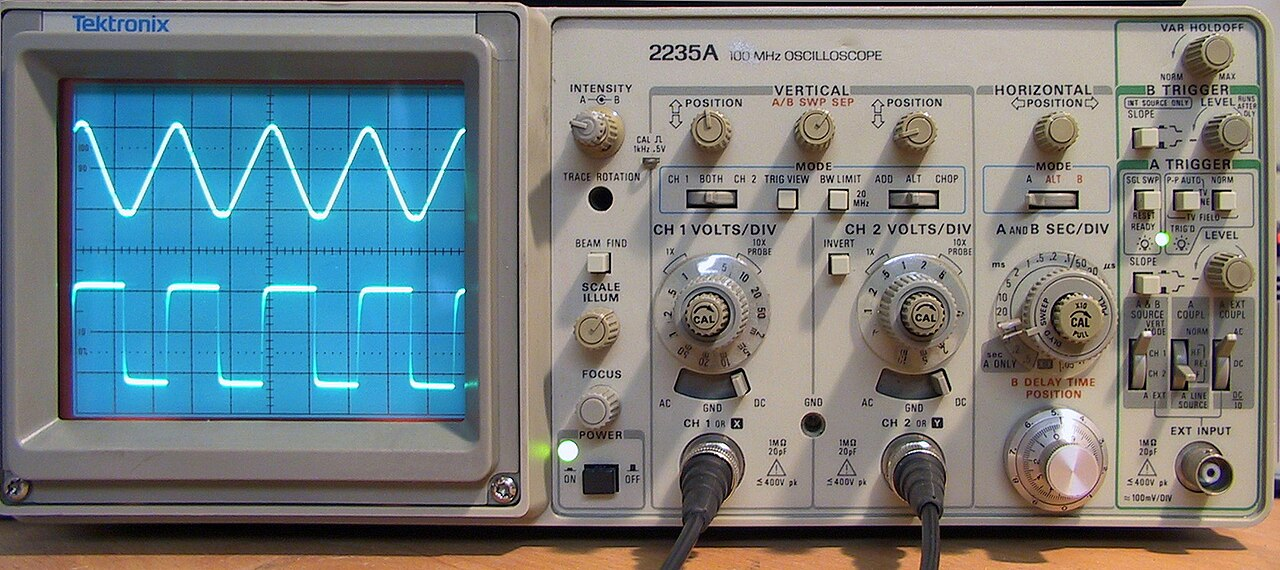
\includegraphics[width=0.60\linewidth]{images/book3/oscilloscope-sine-square.jpg}

{\small Een oscilloscoop met een sinus en een blokgolf: de sinus is het \omterm{def:b1:wave-propagation:signal}{signaal} waarvan dit hoofdstuk leeft, de blokgolf het \omterm{def:b1:wave-propagation:signal}{signaal} dat het volgende hoofdstuk in sinussen ontbindt.}
\end{omfigure}

\section{Het sinusoïdale regime}

\begin{proposition}[Gedwongen sinusoïdaal regime]\label{prop:b1:sinusoidal-impedance:forced}
\index{sinusoïdaal regime}\index{gedwongen regime}
In een \omterm{def:b1:dc-circuits:linear}{lineair netwerk} dat door een sinusvormige bron met \omterm{def:b1:wave-propagation:signal}{hoekfrequentie}
$\omega$ wordt aangedreven, is elke stroom en elke \omterm{def:b1:dc-circuits:voltage}{spanning}, zodra de
\omterm{def:b1:transient-regimes:firstorder}{overgangsverschijnselen} zijn uitgedoofd, een sinus met dezelfde \omterm{def:b1:wave-propagation:signal}{hoekfrequentie} $\omega$, elk met een
eigen \omterm{def:b1:wave-propagation:signal}{amplitude} en fase: $x(t) = X\cos(\omega t + \varphi)$.
\end{proposition}

\begin{proof}
De vergelijkingen van het netwerk zijn lineaire differentiaalvergelijkingen met
constante coëfficiënten; hun algemene oplossing is een particuliere oplossing plus de
oplossingen van de homogene vergelijking, en dat zijn de \omterm{def:b1:transient-regimes:firstorder}{overgangsverschijnselen} van
\cref{ch:b1:transient-regimes}, die uitdoven (elke werkelijke kring heeft enige
weerstand). Er bestaat een sinusvormige particuliere oplossing omdat het
differentiëren van een sinus met frequentie $\omega$ een sinus met
dezelfde frequentie geeft: de vergelijkingen kunnen term voor term worden voldaan --- de
complexe methode hieronder construeert haar expliciet.
\end{proof}

\begin{definition}[Complexe amplitude]\label{def:b1:sinusoidal-impedance:complex}
\index{complexe amplitude}\index{fasor}
Aan de sinus $x(t) = X\cos(\omega t + \varphi)$ koppelt men het
complexe \omterm{def:b1:wave-propagation:signal}{signaal} $\underline{x}(t) = X\eu^{j(\omega t + \varphi)}$, zodat
$x = \Rea(\underline{x})$, en de \emph{complexe \omterm{def:b1:wave-propagation:signal}{amplitude}}
\[
\underline{X} = X\eu^{j\varphi}, \qquad \underline{x}(t) = \underline{X}\,\eu^{j\omega t},
\]
die de \omterm{def:b1:wave-propagation:signal}{amplitude} $X = \abs{\underline{X}}$ en de fase
$\varphi = \arg\underline{X}$ draagt. Hier staat $j$ voor de imaginaire eenheid,
$j^2 = -1$, want de letter $i$ is voor stromen gereserveerd. Getekend als
vector met lengte $X$ onder hoek $\varphi$ is $\underline{X}$ een
\emph{fasor} (Fresnel-vector).
\end{definition}

\begin{proposition}[Regels van de complexe methode]\label{prop:b1:sinusoidal-impedance:rules}
\begin{enumerate}
  \item Lineaire bewerkingen verwisselen met het nemen van het reële deel: de
        \omterm{def:b1:sinusoidal-impedance:complex}{complexe amplitude} van een som is de som van de \omterm{def:b1:sinusoidal-impedance:complex}{complexe amplitudes}.
  \item Differentiëren naar de tijd vermenigvuldigt de \omterm{def:b1:sinusoidal-impedance:complex}{complexe
        amplitude} met $j\omega$; integreren deelt haar door $j\omega$.
  \item De \omterm{thm:b1:dc-circuits:kirchhoff}{wetten van Kirchhoff}, die lineair zijn, gelden voor \omterm{def:b1:sinusoidal-impedance:complex}{complexe amplitudes}.
\end{enumerate}
\end{proposition}

\begin{proof}
$\Rea(\underline a + \underline b) = \Rea\underline a + \Rea\underline b$;
$\dd(\underline X\eu^{j\omega t})/\dd t = j\omega\underline X\eu^{j\omega t}$,
en $\dd x/\dd t = \Rea(\dd\underline x/\dd t)$ omdat differentiëren
reëel-lineair is. Sommen van stromen in een knooppunt en van \omterm{def:b1:dc-circuits:voltage}{spanningen} langs een
maas zijn lineair.
\end{proof}

\begin{example}[Twee sinussen optellen]\label{ex:b1:sinusoidal-impedance:add}
$3\cos\omega t + 4\sin\omega t$: de \omterm{def:b1:sinusoidal-impedance:complex}{complexe amplitudes} zijn $3$ en
$4\eu^{-j\pi/2} = -4j$ (want $\sin\omega t = \cos(\omega t - \pi/2)$);
hun som $3 - 4j$ heeft modulus $5$ en argument $-0.927\ \unit{rad}$:
$5\cos(\omega t - 0.927)$. Geen enkele goniometrische identiteit nodig.
\end{example}

\section{Impedantie}

\begin{definition}[Impedantie, admittantie]\label{def:b1:sinusoidal-impedance:impedance}
\index{impedantie}\index{admittantie}\index{reactantie}
Voor een \omterm{def:b1:dc-circuits:linear}{lineaire tweepool} in het sinusoïdale regime
(verbruikersconventie) is de \emph{impedantie} de verhouding van \omterm{def:b1:sinusoidal-impedance:complex}{complexe amplitudes}
\[
\underline Z = \frac{\underline U}{\underline I} = Z\eu^{j\varphi}
\quad (\text{ohm}),
\]
waarvan de modulus $Z = U/I$ de \omterm{def:b1:wave-propagation:signal}{amplitudes} verbindt en het argument
$\varphi = \varphi_u - \varphi_i$ de fasevoorsprong van de \omterm{def:b1:dc-circuits:voltage}{spanning} op
de stroom is. Haar omgekeerde $\underline Y = 1/\underline Z$ is de
\emph{admittantie} (siemens). Het reële deel van $\underline Z$ is haar
weerstand, het imaginaire deel haar \emph{reactantie}.
\end{definition}

\begin{proposition}[Impedanties van R, L, C]\label{prop:b1:sinusoidal-impedance:rlc}
\[
\underline Z_R = R, \qquad \underline Z_L = jL\omega, \qquad
\underline Z_C = \frac{1}{jC\omega} = -\frac{j}{C\omega} .
\]
Een weerstand houdt \omterm{def:b1:dc-circuits:voltage}{spanning} en stroom in fase; in een spoel loopt de \omterm{def:b1:dc-circuits:voltage}{spanning}
$\pi/2$ voor op de stroom; in een condensator loopt zij $\pi/2$ achter. Bij lage
frequentie nadert een spoel een draad en een condensator een open keten; bij
hoge frequentie andersom.
\end{proposition}

\begin{proof}
$u = Ri$; $u = L\,\dd i/\dd t \to \underline U = jL\omega\,\underline I$;
$i = C\,\dd u/\dd t \to \underline I = jC\omega\,\underline U$. De
argumenten van $1$, $j$ en $-j$ zijn $0$, $\pi/2$, $-\pi/2$.
\end{proof}

\begin{proposition}[Schakeling; delers; stellingen]\label{prop:b1:sinusoidal-impedance:assoc}
\omterm{def:b1:sinusoidal-impedance:impedance}{Impedanties} in serie tellen op; \omterm{def:b1:sinusoidal-impedance:impedance}{admittanties} parallel tellen op; de spannings- en
\omterm{prop:b1:dc-circuits:dividers}{stroomdelers}, de stellingen van Thévenin en Norton, de superpositie en
de stelling van Millman uit \cref{ch:b1:dc-circuits} gelden alle met \omterm{def:b1:sinusoidal-impedance:complex}{complexe
amplitudes} en \omterm{def:b1:sinusoidal-impedance:impedance}{impedanties} in plaats van reële \omterm{def:b1:dc-circuits:voltage}{spanningen}, stromen en
weerstanden.
\end{proposition}

\begin{proof}
Elk bewijs in \cref{ch:b1:dc-circuits} gebruikte alleen de \omterm{thm:b1:dc-circuits:kirchhoff}{wetten van Kirchhoff} en
de lineariteit van $u = Ri$, en beide gelden in complexe vorm.
\end{proof}

\begin{example}[De RC-deler]\label{ex:b1:sinusoidal-impedance:rcdivider}
Een weerstand $R$ en een condensator $C$ in serie over $\underline E$, met de
uitgang over $C$: $\underline U_C = \underline E\,\dfrac{1/jC\omega}
{R + 1/jC\omega} = \dfrac{\underline E}{1 + jRC\omega}$. \omterm{def:b1:wave-propagation:signal}{Amplitude}
$E/\sqrt{1 + (RC\omega)^2}$, fase $-\arctan(RC\omega)$: volledige
doorlating bij lage frequentie, $1/\sqrt2$ en $-45^\circ$ bij
$\omega = 1/RC$, en daarboven een daling als $1/\omega$ --- een laagdoorlaatfilter, het
onderwerp van \cref{ch:b1:filters-transfer-functions}.
\end{example}

\section{De RLC-kring in serie: resonantie}

\begin{theorem}[Stroomresonantie]\label{thm:b1:sinusoidal-impedance:resonance}
\index{resonantie}\index{resonantie!stroom}\index{bandbreedte}
Een weerstand $R$, een spoel $L$ en een condensator $C$ in serie over
$e(t) = E\cos\omega t$ voeren de stroom met \omterm{def:b1:sinusoidal-impedance:complex}{complexe amplitude}
\[
\underline I = \frac{E}{R + j\left(L\omega - \dfrac{1}{C\omega}\right)},
\qquad
I = \frac{E}{\sqrt{R^2 + \left(L\omega - \dfrac{1}{C\omega}\right)^2}},
\qquad
\varphi_i = -\arctan\frac{L\omega - 1/C\omega}{R} .
\]
De \omterm{def:b1:wave-propagation:signal}{amplitude} is maximaal, $I_{\max} = E/R$, met stroom en \omterm{def:b1:dc-circuits:voltage}{spanning} in
fase, bij de \emph{resonantie} $\omega_0 = 1/\sqrt{LC}$. Met
$Q = L\omega_0/R = 1/(RC\omega_0)$ en $x = \omega/\omega_0$ geldt
\[
\frac{I}{I_{\max}} = \frac{1}{\sqrt{1 + Q^2\left(x - \dfrac1x\right)^2}} ,
\]
en de \emph{bandbreedte} --- het interval van $\omega$ waarop
$I \geq I_{\max}/\sqrt2$ --- bedraagt
\[
\Delta\omega = \omega_2 - \omega_1 = \frac{\omega_0}{Q} = \frac{R}{L} .
\]
\end{theorem}

\begin{proof}
\omterm{def:b1:sinusoidal-impedance:impedance}{Impedanties} in serie tellen op: $\underline Z = R + jL\omega + 1/jC\omega$, en
$\underline I = \underline E/\underline Z$. De modulus is het grootst wanneer
de \omterm{def:b1:sinusoidal-impedance:impedance}{reactantie} $L\omega - 1/C\omega$ verdwijnt, dus bij $\omega_0$.
Ontbind $L\omega - 1/C\omega = L\omega_0(x - 1/x)$ en deel door $R$:
$L\omega_0/R = Q$. Aan de randen van de band geldt $Q(x - 1/x) = \pm 1$, dus
$x^2 \mp x/Q - 1 = 0$, waarvan de positieve wortels $x_{1,2} = \mp\frac{1}{2Q}
+ \sqrt{1 + \frac{1}{4Q^2}}$ zijn; hun verschil is $1/Q$.
\end{proof}

\begin{omfigure}
\begin{tikzpicture}
\begin{axis}[omaxis, width=7.6cm, height=5.4cm, xlabel={$\omega/\omega_0$}, ylabel={$I/I_{\max}$},
    xmin=0, xmax=2.1, ymin=0, ymax=1.45, xtick={0.5,1,1.5,2}, ytick={0.5,0.707,1},
    yticklabels={$0.5$,$\frac{1}{\sqrt2}$,$1$},
    legend style={at={(0.97,0.97)}, anchor=north east, font=\footnotesize, draw=none, fill=none}]
  \addplot[omProp, thick, domain=0.05:2.1, samples=300] {1/sqrt(1 + (1*(x - 1/x))^2)};
  \addlegendentry{$Q = 1$}
  \addplot[omDef, thick, domain=0.05:2.1, samples=300] {1/sqrt(1 + (3*(x - 1/x))^2)};
  \addlegendentry{$Q = 3$}
  \addplot[omThm, thick, domain=0.05:2.1, samples=500] {1/sqrt(1 + (10*(x - 1/x))^2)};
  \addlegendentry{$Q = 10$}
  \draw[dashed, omExo] (axis cs:0,0.707) -- (axis cs:2.1,0.707);
\end{axis}
\end{tikzpicture}\qquad
\begin{tikzpicture}
\begin{axis}[omaxis, width=7.0cm, height=5.4cm, xlabel={$\omega/\omega_0$}, ylabel={$\varphi_i$},
    xmin=0, xmax=2.1, ymin=-1.8, ymax=1.8, xtick={0.5,1,1.5,2}, ytick={-1.5708,0,1.5708},
    yticklabels={$-\frac{\pi}{2}$,$0$,$\frac{\pi}{2}$}]
  \addplot[omProp, thick, domain=0.05:2.1, samples=300] {-rad(atan(1*(x - 1/x)))};
  \addplot[omDef, thick, domain=0.05:2.1, samples=300] {-rad(atan(3*(x - 1/x)))};
  \addplot[omThm, thick, domain=0.05:2.1, samples=500] {-rad(atan(10*(x - 1/x)))};
\end{axis}
\end{tikzpicture}

{\small RLC in serie: \omterm{def:b1:wave-propagation:signal}{amplitude} van de stroom (links) en haar fase
ten opzichte van de bron (rechts) tegen $\omega/\omega_0$, voor
$Q = 1, 3, 10$. De piek wordt smaller naarmate $Q$ groeit ($\Delta\omega =
\omega_0/Q$); onder de resonantie is de kring capacitief (de stroom
loopt voor), erboven inductief (de stroom loopt achter).}
\end{omfigure}

\begin{omfigure}
\begin{tikzpicture}[font=\small, x=1cm, y=1cm, >=Stealth]
  % phasors for RLC at omega above resonance: UR along I, UL +90, UC -90
  \draw[->, thick, omExo] (0,0) -- (2.6,0) node[right] {$\underline I$};
  \draw[->, very thick, omProp] (0,0) -- (1.6,0) node[midway, below] {$\underline U_R = R\underline I$};
  \draw[->, very thick, omDef] (1.6,0) -- (1.6,2.4) node[left, pos=0.8] {$\underline U_L = jL\omega\underline I$};
  \draw[->, very thick, omDef!60] (1.78,2.4) -- (1.78,1.1) node[right, midway] {$\underline U_C = \underline I/jC\omega$};
  \draw[->, very thick, omThm] (0,0) -- (1.6,1.1) node[midway, above left, xshift=-1pt] {$\underline E$};
  \draw (0.6,0) arc (0:34.5:0.6); \node at (0.85,0.2) {$\varphi$};
\end{tikzpicture}

{\small Fasordiagram van de RLC in serie boven de resonantie: $\underline U_R$
langs $\underline I$, $\underline U_L$ een kwartslag vooruit, $\underline U_C$
een kwartslag achteruit; hun som $\underline E$ loopt op de stroom voor met
$\varphi$. Bij resonantie heffen $\underline U_L$ en $\underline U_C$ elkaar op en is
$\underline E = \underline U_R$.}
\end{omfigure}

\begin{proposition}[Spanningsopslingering]\label{prop:b1:sinusoidal-impedance:overvoltage}
\index{resonantie!spanning}\index{overspanning}
Bij resonantie hebben de \omterm{def:b1:dc-circuits:voltage}{spanningen} over de spoel en de condensator dezelfde
\omterm{def:b1:wave-propagation:signal}{amplitude} $QE$ en tegengestelde fasen: voor $Q \gg 1$ draagt de condensator
een \omterm{def:b1:dc-circuits:voltage}{spanning} die $Q$ keer groter is dan die van de bron. De \omterm{def:b1:wave-propagation:signal}{amplitude}
$U_C(\omega)$ zelf piekt, voor $Q > 1/\sqrt2$, bij $\omega_r =
\omega_0\sqrt{1 - 1/2Q^2}$, iets onder $\omega_0$, met
$U_{C,\max} = QE/\sqrt{1 - 1/4Q^2}$.
\end{proposition}

\begin{proof}
Bij $\omega_0$ is $\underline U_C = \underline I/jC\omega_0 = -jQE$ en
$\underline U_L = jL\omega_0\underline I = jQE$, aangezien $I = E/R$. In het
algemeen is $U_C = I/C\omega = E/\sqrt{(1 - x^2)^2 + x^2/Q^2}$ (vermenigvuldig
teller en noemer met $1/C\omega_0$); het kwadraat van de noemer
is $(1 - x^2)^2 + x^2/Q^2$, kwadratisch in $x^2$ en minimaal bij $x^2 =
1 - 1/2Q^2$ wanneer dat positief is, met minimum $1/Q^2 - 1/4Q^4$.
\end{proof}

\begin{example}[Een radio afstemmen]\label{ex:b1:sinusoidal-impedance:radio}
Een spoel $L = \qty{200}{\micro H}$ en een regelbare condensator: $C =
\qty{127}{pF}$ stemt af op $f_0 = \qty{1.00}{MHz}$. Met de draadweerstand
van de spoel $R = \qty{12.6}{\ohm}$ is $L\omega_0 = \qty{1257}{\ohm}$ en
$Q = 100$: bandbreedte $\Delta f = f_0/Q = \qty{10}{kHz}$ --- de breedte van
een AM-kanaal --- en de \qty{10}{\micro V} die een verre zender induceert
wordt $QE = \qty{1}{mV}$ over de condensator, gratis en voor niets.
De weekendopgave bouwt deze ontvanger.
\end{example}

\begin{remark}[Waarom weer $Q$]\label{rem:b1:sinusoidal-impedance:Q}
De $Q$ van dit hoofdstuk is de $Q$ van \cref{ch:b1:transient-regimes}:
de kring die na een tik ongeveer $Q$ trillingen nagalmt, is dezelfde
die over een band van $\omega_0/Q$ breed resoneert wanneer zij wordt aangedreven. Beide
drukken één verhouding uit: $2\pi$ maal de opgeslagen energie gedeeld door de
per periode gedissipeerde energie (\cref{exo:b1:sinusoidal-impedance:12}). Een
scherpe resonantie en een lange nagalm zijn dezelfde eigenschap, en dat geldt ook voor de
trage reactie: een filter met bandbreedte $\Delta\omega$ heeft een tijd van de
orde $1/\Delta\omega$ nodig om zich in te stellen.
\end{remark}

\section{Vermogen in het sinusoïdale regime}

\begin{definition}[Effectieve waarde]\label{def:b1:sinusoidal-impedance:rms}
\index{effectieve waarde}\index{rms-waarde}
De \emph{effectieve waarde} (rms) van een periodiek
\omterm{def:b1:wave-propagation:signal}{signaal} $x(t)$ is $X_{\mathrm{rms}} = \sqrt{\langle x^2\rangle}$, de
wortel uit het tijdgemiddelde van $x^2$ over een periode. Voor een sinus
met \omterm{def:b1:wave-propagation:signal}{amplitude} $X$ is $X_{\mathrm{rms}} = X/\sqrt2$. De \qty{230}{V} van het
lichtnet is een effectieve waarde; de \omterm{def:b1:wave-propagation:signal}{amplitude} is \qty{325}{V}.
\end{definition}

\begin{theorem}[Gemiddeld vermogen]\label{thm:b1:sinusoidal-impedance:power}
\index{gemiddeld vermogen}\index{arbeidsfactor}\index{blindvermogen}
Een tweepool met $u = U\cos\omega t$ en $i = I\cos(\omega t - \varphi)$
(verbruikersconventie) ontvangt het ogenblikkelijke vermogen $p = ui$, met
gemiddelde
\[
P = \tfrac12\,UI\cos\varphi = U_{\mathrm{rms}}I_{\mathrm{rms}}\cos\varphi
= \tfrac12\Rea\!\big(\underline U\,\underline I^{\,*}\big) = \tfrac12\Rea(\underline Z)\,I^2,
\]
waarin $\cos\varphi$ de \emph{arbeidsfactor} is. Een weerstand ontvangt
$\tfrac12 RI^2 = RI_{\mathrm{rms}}^2$; een ideale spoel of condensator
($\varphi = \pm\pi/2$) ontvangt geen \omterm{thm:b1:sinusoidal-impedance:power}{gemiddeld vermogen} --- zij slaat energie op
gedurende een halve periode en geeft die in de andere helft terug.
\end{theorem}

\begin{proof}
$p = UI\cos\omega t\cos(\omega t - \varphi) = \tfrac12 UI[\cos\varphi +
\cos(2\omega t - \varphi)]$; de tweede term middelt tot nul. Met
$\underline U = U$ en $\underline I = I\eu^{-j\varphi}$ is
$\underline U\,\underline I^* = UI\eu^{j\varphi}$, waarvan het reële deel
$UI\cos\varphi$ is; en $\underline U = \underline Z\,\underline I$ geeft
$\underline U\,\underline I^* = \underline Z I^2$.
\end{proof}

\begin{omfigure}
\begin{tikzpicture}
\begin{axis}[omaxis, axis x line=bottom, width=11.5cm, height=5cm, xlabel={$t/T$}, ylabel={$p$},
    xmin=0, xmax=2, ymin=-0.5, ymax=1.15, xtick={0.5,1,1.5,2}, ytick={0,0.5,1},
    yticklabels={$0$,$P$,$UI$}]
  \addplot[omDef, thick, domain=0:2, samples=300] {cos(deg(2*pi*x))*cos(deg(2*pi*x) - 60)};
  \addplot[omThm, thick, dashed, domain=0:2, samples=2] {0.25};
  \addplot[omExo, dashed, domain=0:2, samples=2] {0};
  \node[omDef, font=\footnotesize] at (axis cs:1.62,0.95) {$p(t) = ui$, $\varphi = 60^\circ$};
  \node[omThm, font=\footnotesize] at (axis cs:0.5,0.95) {gemiddelde $P = \tfrac12 UI\cos\varphi$ (streepjes)};
\end{axis}
\end{tikzpicture}

{\small Ogenblikkelijk vermogen dat een tweepool ontvangt met $60^\circ$
faseachterstand tussen stroom en \omterm{def:b1:dc-circuits:voltage}{spanning}: het pulseert met $2\omega$, duikt onder nul
(energie terug naar de bron) en middelt tot $\tfrac12 UI\cos\varphi$
--- hier de helft van wat het in fase zou zijn.}
\end{omfigure}

\begin{example}[De arbeidsfactor verbeteren]\label{ex:b1:sinusoidal-impedance:pf}
Een werkplaatsmotor op \qty{230}{V} effectief neemt \qty{2.0}{kW} op met
$\cos\varphi = 0.70$ (inductief): $I_{\mathrm{rms}} = 2000/(230 \times
0.70) = \qty{12.4}{A}$, tegen \qty{8.7}{A} als de arbeidsfactor
$1$ was --- de extra stroom verwarmt de kabels van het net voor niets, vandaar
de boete. Een condensator parallel levert de energieschommelingen van de spoel
ter plaatse per kwartperiode: het \emph{blindvermogen} $P\tan\varphi =
\qty{2.0}{kvar}$ vraagt $C = P\tan\varphi/(\omega U_{\mathrm{rms}}^2)
\approx \qty{120}{\micro F}$ bij \qty{50}{Hz}, en de netstroom zakt
naar \qty{8.7}{A}.
\end{example}

\section{Oefeningen}

\begin{exercise}[$\star$]\label{exo:b1:sinusoidal-impedance:1}
Geef de \omterm{def:b1:sinusoidal-impedance:complex}{complexe amplitude} van $u = 5\cos(\omega t + \pi/3)$ (V), in
polaire en in cartesische vorm. Schrijf met \omterm{def:b1:sinusoidal-impedance:complex}{complexe amplitudes} $3\cos\omega t
+ 4\sin\omega t$ als één cosinus.
\end{exercise}

\begin{exercise}[$\star$]\label{exo:b1:sinusoidal-impedance:2}
Bereken de \omterm{def:b1:sinusoidal-impedance:impedance}{impedantie} van $R = \qty{100}{\ohm}$, $L = \qty{0.10}{H}$ en
$C = \qty{10}{\micro F}$ bij \qty{50}{Hz} en bij \qty{1.0}{kHz}. Geef de
modulus en de fase van de \omterm{def:b1:sinusoidal-impedance:impedance}{impedantie} van $R$ en $L$ in serie bij
\qty{50}{Hz}.
\end{exercise}

\begin{exercise}[$\star$]\label{exo:b1:sinusoidal-impedance:3}
Het lichtnet is \qty{230}{V} effectief: hoe groot is de \omterm{def:b1:wave-propagation:signal}{amplitude}? Een kachel van
\qty{2.0}{kW}: effectieve en piekstroom. Toon aan dat het \omterm{thm:b1:sinusoidal-impedance:power}{gemiddelde vermogen} in een weerstand
$RI_{\mathrm{rms}}^2$ is.
\end{exercise}

\begin{exercise}[$\star$]\label{exo:b1:sinusoidal-impedance:4}
RLC in serie: $L = \qty{10}{mH}$, $C = \qty{100}{nF}$, $R = \qty{100}{\ohm}$,
$E = \qty{1.0}{V}$. Geef $f_0$, $Q$, de bandbreedte in hertz en de
stroomamplitude bij resonantie.
\end{exercise}

\begin{exercise}[$\star\star$]\label{exo:b1:sinusoidal-impedance:5}
RC-deler, uitgang over $C$: $R = \qty{1.0}{k\ohm}$, $C = \qty{159}{nF}$.
Bij welke frequentie is de uitgang $1/\sqrt2$ van de ingang? Geef de
amplitudeverhouding en de fase bij \qty{1.0}{kHz} en bij \qty{10}{kHz}.
\end{exercise}

\begin{exercise}[$\star\star$]\label{exo:b1:sinusoidal-impedance:6}
Bij een zekere frequentie heeft een RLC in serie $R = \qty{100}{\ohm}$, $L\omega =
\qty{250}{\ohm}$, $1/C\omega = \qty{100}{\ohm}$ en $E = \qty{1.0}{V}$.
Bereken $\underline Z$, de \omterm{def:b1:wave-propagation:signal}{amplitude} en de fase van de stroom en de drie
spanningsamplitudes; teken het fasordiagram. Zit de kring boven of
onder de resonantie?
\end{exercise}

\begin{exercise}[$\star\star$]\label{exo:b1:sinusoidal-impedance:7}
Radio: $L = \qty{200}{\micro H}$, $C$ regelbaar van \qty{50}{} tot
\qty{500}{pF}. Bepaal het frequentiebereik, de capaciteit voor
\qty{1.00}{MHz}, en met $Q = 100$ de bandbreedte en de verzwakking
(amplitudeverhouding) van een zender op \qty{9}{kHz} afstand. Bij een antenne-emk van
\qty{10}{\micro V}: \omterm{def:b1:dc-circuits:voltage}{spanning} over $C$ bij resonantie?
\end{exercise}

\begin{exercise}[$\star\star$]\label{exo:b1:sinusoidal-impedance:8}
Leid de twee halfvermogenfrequenties van de RLC in serie af en toon aan dat
hun verschil $\omega_0/Q$ is en hun product $\omega_0^2$.
\end{exercise}

\begin{exercise}[$\star\star$]\label{exo:b1:sinusoidal-impedance:9}
Een motor op \qty{230}{V} effectief, \qty{50}{Hz}, neemt \qty{2.0}{kW} op met
$\cos\varphi = 0.70$. Bereken de effectieve stroom, het blindvermogen, de
capaciteit die er parallel voor zorgt dat de arbeidsfactor $1$ wordt, en de
nieuwe stroom. De voedingskabel heeft \qty{0.50}{\ohm}: joulewarmte ervóór
en erna.
\end{exercise}

\begin{exercise}[$\star\star\star$]\label{exo:b1:sinusoidal-impedance:10}
RLC parallel gevoed door een \omterm{def:b1:dc-circuits:sources}{stroombron}: schrijf de \omterm{def:b1:sinusoidal-impedance:impedance}{admittantie} op, toon aan dat
de \omterm{def:b1:dc-circuits:voltage}{spanning} maximaal is bij $\omega_0 = 1/\sqrt{LC}$ en daar gelijk is aan $RI$,
en dat de bandbreedte $\Delta\omega = 1/RC$ bedraagt, dus $Q =
R\sqrt{C/L}$. Getallen: $R = \qty{10}{k\ohm}$, $L = \qty{1.0}{mH}$,
$C = \qty{1.0}{nF}$.
\end{exercise}

\begin{exercise}[$\star\star\star$]\label{exo:b1:sinusoidal-impedance:11}
Toon aan dat de condensatorspanning van een RLC in serie $U_C = E/\sqrt{(1 -
x^2)^2 + x^2/Q^2}$ is, dat zij piekt bij $x_r = \sqrt{1 - 1/2Q^2}$ als
$Q > 1/\sqrt2$, en bereken $x_r$ en $U_{C,\max}/E$ voor $Q = 3.16$.
Wat gebeurt er voor $Q < 1/\sqrt2$?
\end{exercise}

\begin{exercise}[$\star\star\star$]\label{exo:b1:sinusoidal-impedance:12}
Toon aan dat bij resonantie van een RLC in serie de totale opgeslagen energie
$\tfrac12 Li^2 + \tfrac12 Cu_C^2$ constant en gelijk aan $\tfrac12 LI^2$ is,
bereken de per periode in $R$ gedissipeerde energie en bewijs dat
$2\pi\,(\text{opgeslagen})/(\text{gedissipeerd per periode}) = Q$.
\end{exercise}

\begin{omfigure}

\includegraphics[width=0.55\linewidth]{images/book3/ai/b3-08-vintage-radio-tuning.jpg}

{\small Een buizenradio afstemmen: aan de knop draaien verandert een condensator, de condensator bepaalt de resonantiefrequentie van een $LC$-kring, en de zender waarvan de frequentie past is de zender die je hoort --- de weekendopgave.}
\end{omfigure}

\section{Probleem: De resonante radio-ontvanger}

\begin{problem}[{Weekendopgave --- een spoel, een regelbare condensator en
een antenne: hoe een serieresonantie één zender uit honderd oppikt,
haar zwakke signaal met honderd vermenigvuldigt, en waarom zij niet
willekeurig selectief kan worden gemaakt}]
\label{pb:b1:sinusoidal-impedance:1}
De antenne wordt gemodelleerd als een ideale sinusvormige emk $e(t) = E\cos\omega t$
in serie met een spoel $L = \qty{200}{\micro H}$, waarvan de draad
weerstand $R = \qty{12.6}{\ohm}$ heeft, en een regelbare condensator $C$. De
ontvanger leest de \omterm{def:b1:dc-circuits:voltage}{spanning} over $C$. Later (deel IV) wordt de eigen weerstand
$R_a = \qty{50}{\ohm}$ van de antenne meegerekend.

\medskip
\noindent\textbf{Deel I --- De resonante stroom.}
\begin{enumerate}
  \item Schrijf de complexe \omterm{def:b1:sinusoidal-impedance:impedance}{impedantie} van de serieschakeling op.
  \item Geef de \omterm{def:b1:sinusoidal-impedance:complex}{complexe amplitude} van de stroom, dan haar \omterm{def:b1:wave-propagation:signal}{amplitude}
        $I(\omega)$ en haar fase $\varphi_i(\omega)$ ten opzichte van $e$.
  \item Toon aan dat $I$ maximaal is bij $\omega_0 = 1/\sqrt{LC}$; geef
        $I_{\max}$ en de fase op dat moment.
  \item Welke capaciteit stemt af op $f_0 = \qty{1.000}{MHz}$? Bereken
        $L\omega_0$.
  \item Definieer $Q = L\omega_0/R$ en bereken het.
  \item Toon aan dat $I/I_{\max} = 1/\sqrt{1 + Q^2(x - 1/x)^2}$ met
        $x = \omega/\omega_0$.
  \item Geef het teken van $\varphi_i$ onder en boven de resonantie en
        duid het (capacitief of inductief gedrag).
\end{enumerate}

\medskip
\noindent\textbf{Deel II --- Selectiviteit.}
\begin{enumerate}[resume]
  \item Schrijf de voorwaarde op die de twee frequenties bepaalt waarbij
        $I = I_{\max}/\sqrt2$.
  \item Los haar op en toon aan dat $\Delta\omega = \omega_2 - \omega_1 =
        \omega_0/Q$.
  \item Bereken de bandbreedte $\Delta f$ van deze ontvanger.
  \item Een tweede zender zendt uit op \qty{1.010}{MHz}, een derde op
        \qty{1.020}{MHz}: bereken de amplitudeverhouding $I/I_{\max}$ voor
        elk, en de bijbehorende vermogensverhouding in decibel.
  \item AM-zenders liggen \qty{9}{} tot \qty{10}{kHz} uit elkaar. Is de
        ontvanger selectief genoeg? Wat zou hem verbeteren?
  \item De condensator kan tussen \qty{50}{} en \qty{500}{pF} worden gezet:
        welke frequentieband bestrijkt de ontvanger?
\end{enumerate}

\medskip
\noindent\textbf{Deel III --- Spanningsopslingering.}
\begin{enumerate}[resume]
  \item Druk de \omterm{def:b1:sinusoidal-impedance:complex}{complexe amplitude} van de condensatorspanning uit en toon aan
        dat haar \omterm{def:b1:wave-propagation:signal}{amplitude} bij resonantie $QE$ is.
  \item De emk van de antenne is $E = \qty{10}{\micro V}$: bereken $I_{\max}$
        en de condensatorspanning bij resonantie. Becommentarieer.
  \item Toon aan dat de spoelspanning bij resonantie dezelfde \omterm{def:b1:wave-propagation:signal}{amplitude} heeft en in
        tegenfase is met de condensatorspanning: wat ``ziet'' de bron?
  \item Bereken de energie die bij resonantie in de kring is opgeslagen en de
        energie die per periode wordt gedissipeerd; ga na dat hun verhouding maal
        $2\pi$ gelijk is aan $Q$.
  \item Wat is, volgens \cref{ch:b1:transient-regimes}, de \omterm{def:b1:transient-regimes:firstorder}{tijdconstante}
        $\tau = 2Q/\omega_0$ van deze kring? Waarom vervormt een zeer hoge $Q$
        uiteindelijk spraak en muziek (bandbreedte van audio:
        ongeveer \qty{5}{kHz} voor AM)?
  \item Als de draadweerstand van de spoel verdubbelde (dunner draad), hoe zouden
        $Q$, de bandbreedte en de condensatorspanning dan veranderen?
\end{enumerate}

\medskip
\noindent\textbf{Deel IV --- De weerstand van de antenne, en het vermogen.}
\begin{enumerate}[resume]
  \item Herbereken met $R_a = \qty{50}{\ohm}$ in serie de waarde van $Q$, de
        bandbreedte en de condensatorspanning voor $E = \qty{10}{\micro V}$.
        Trek een conclusie.
  \item Bereken het \omterm{thm:b1:sinusoidal-impedance:power}{gemiddelde vermogen} dat de emk van de antenne bij
        resonantie levert en de fractie die in $R_a$ wordt gedissipeerd.
  \item De stelling van het maximale vermogen zou een belastingsweerstand vragen die gelijk is
        aan $R_a$: waarom botst dat doel met de selectiviteit?
  \item Werkelijke ontvangers verbinden de antenne met een aftakking op de spoel, of
        via een kleine koppelcondensator. Leg kwalitatief uit wat dat
        oplevert.
  \item Bereken met $P = \tfrac12 UI\cos\varphi$ de arbeidsfactor bij
        de twee halfvermogenfrequenties en verklaar de naam
        ``halfvermogen''.
  \item Vat het ontwerp samen: wat $Q$ oplevert, wat het kost, en de
        waarde die voor een ontvanger op \qty{1}{MHz} met kanalen van \qty{10}{kHz}
        wordt gekozen.
\end{enumerate}
\end{problem}
